\documentclass[a4paper,12pt]{article} 
\usepackage[utf8]{inputenc} 
\usepackage[T1]{fontenc} 
%\usepackage{graphicx}
\usepackage{lmodern,textcomp} 
\usepackage[frenchb]{babel} 
\usepackage{color}
\usepackage{eso-pic}
\usepackage{upquote}
\usepackage{courier}
\usepackage{caption}
\usepackage{listings}
\usepackage{fancyhdr}
\usepackage{caption}
\usepackage{pdflscape}

\usepackage{amssymb}
\usepackage[table]{xcolor}
\definecolor{gris}{gray}{0.75}
\definecolor{bleup}{HTML}{258EE9}


%\renewcommand*\familydefault{\ttdefault} %% Only if the base font of the document is to be typewriter style
%\renewcommand{\rmdefault}{ptm}


\usepackage[
   pdfauthor={Ludovic Terrier & Arnaud Goulut},
   pdftitle={RE12 - TP1},
   ]{hyperref}
  
\hypersetup{
    %bookmarks=true,         % show bookmarks bar?
    unicode=false,          % non-Latin characters in Acrobat’s bookmarks
    pdffitwindow=false,     % window fit to page when opened
    pdfstartview={FitH},    % fits the width of the page to the window
    pdftitle={Rapport de stage TN09},    % title
    pdfauthor={Ludovic Terrier},     % author
    pdfsubject={Subject},   % subject of the document
    pdfcreator={Ludovic Terrier},   % creator of the document
    pdfkeywords={TN09, rapport, Com-IP}, % list of keywords
    pdfnewwindow=true,      % links in new window
    colorlinks=true,       % false: boxed links; true: colored links
   linkcolor= redbrick, %couleur des liens internes
    %citecolor=green,        % color of links to bibliography
    filecolor=magenta,      % color of file links
   % urlcolor=cyan           % color of external links
}
  
  
\usepackage[pdftex]{graphicx}

%\usepackage{titlesec}
%\titleformat{\section}[frame] {\normalfont} {\filright
%\footnotesize
%\enspace\textbf{\thesection}\enspace} {8pt} {\Large\bfseries\filcenter}

%% Je contrôle la taille de ma zone imprimée...
\usepackage{anysize}
%% ...en définissants les marges {gauche}{droite}{haute}{basse}
\marginsize{25mm}{15mm}{10mm}{15mm}

\begin{document}

\title{La configuration réseau sous Linux}
\author{Ludovic Terrier et Arnaud Goulut}
\date{Mars 2010}
\maketitle


%\tableofcontents

\thispagestyle{empty}
\newpage

%%%%%%%%%%%%%%%%%%%%%%%%%%%%%%%%%%%  1ère page


%%%%%%%%%%%%%%%%%%%%%%%%%%%%%%%%%%% 1ère partie
\section{Partie 1}

\subsection{Question 1}
\begin{figure}[!h]
\begin{center}
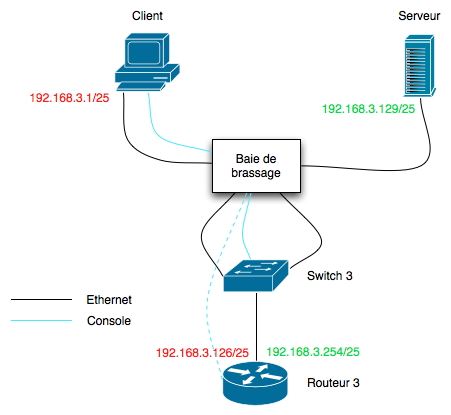
\includegraphics[height=11cm]{Diag.png}
\caption{Présentation du réseau configuré au cours du TP.}
\label{fig:do}
\end{center}
\end{figure}
\subsection{Question 2}


\begin{center}
\rowcolors{1}{gris}{}
\begin{tabular}{|c|c|}
  \hline
 \multicolumn{2}{|c|}{\cellcolor{bleup}Réseau du client} \\
  \hline
  NetID & 192.168.3.0 \\
  Masque & /25  \\
  Plage d'adresse & 192.168.3.0 - 192.168.3.127\\
  1\up{ere} adresse machine & 192.168.3.1\\
  Dernière adresse machine & 192.168.2.126\\
  Nombre de machines potentiel & 126\\
  Broadcast & 192.168.3.127\\
  \hline
\end{tabular}
\end{center}

\begin{center}
\rowcolors{1}{gris}{}
\begin{tabular}{|c|c|}
  \hline
  \rowcolor{orangec} \multicolumn{2}{|c|}{\cellcolor{bleup}Réseau du seveur (DMZ)} \\
  \hline
  NetID & 192.168.3.128 \\
  Masque & /25  \\
  Plage d'adresse & 192.168.3.128 - 192.168.3.255\\
  1\up{ere} adresse machine & 192.168.3.129\\
  Dernière adresse machine& 192.168.3.254\\
  Nombre de machines potentiel & 126\\
  Broadcast & 192.168.3.255\\
  \hline
\end{tabular}
\end{center}

\begin{center}
\rowcolors{1}{gris}{}
\begin{tabular}{|c|c|}
  \hline
  \rowcolor{orangec} \multicolumn{2}{|c|}{\cellcolor{bleup}Réseau de transport} \\
  \hline
  NetID & 172.16.3.0 \\
  Masque & /30  \\
  Plage d'adresse & 172.16.3.0 - 172.16.3.3\\
  1\up{ere} adresse machine & 172.16.3.1\\
  Dernière adresse machine&  172.16.3.2\\
  Nombre de machines potentiel & 2\\
  Broadcast & 172.16.3.3\\
  \hline
\end{tabular}
\end{center}

\paragraph{}Dans les réseaux du serveur et du client on utilise un seul réseau (192.168.3.0) de classe C. Cependant pour en faire deux réseaux distincts on le scinde à l'aide du masque : $\mathtt{/25}$. Ceci signifie que les 25 premiers bits de chaque adresse IP utilisée sur le réseau correspondra au NetID et les 7 derniers au HostID. On obtient donc 2 sous-réseaux ayant pour adresse respective : 192.168.3.0 et 192.168.3.128.

\paragraph{}Dans le cas du réseau de transport, nous avons un réseau 172.16.3.0, qui contiendra seulement deux machines. C'est pourquoi on peut se permettre d'utiliser un masque $\mathtt{/30}$ qui, appliqué à notre réseau de départ donne 4 adresses :
\begin{itemize}
\item deux adresses à utiliser pour des hosts,
\item une pour le broadcast,
\item une pour le NetID.
\end{itemize}


\subsection{Question 3}

Pour l'administration de matériel réseaux on préfère utiliser un port console dédié. Ceci afin d'assurer l'accès à l'équipement en cas d'une mauvaise manipulation, qui le rendrait inaccessible via ses interfaces réseaux (Ethernet dans le cadre des TPs) ou dans le cas d'une congestion du réseau. On s'affranchit alors de tout problème d'adressage.\\

Cette interface est un port série (avec connectique RJ45 et DB9)


\section{Partie 2}
\subsection{Configuration du switch}

Le switch peut-être logiquement séparé en deux grâce aux Virtual Local Area Networks (VLANs). Une différenciation des deux VLANs peut se faire par ports, ce qui se voit dans le fichier de configuration des switchs, seul le port \textit{FastEthernet0/2} est attribué à un VLAN :

\begin{center}
\fbox{
    \begin{minipage}{8cm}
    \hspace{2cm}\vdots\\
    {\small interface FastEthernet0/2}\\                       
    {\small switchport access vlan 2}
     
     
     \hspace{2cm}\vdots
     \end{minipage}
}
 \end{center}
 
Ce qui peut vouloir dire que l'ensemble des autres ports sont dans le même VLAN par défaut.

\subsection{Configuration du routeur}
\paragraph{}Le switch de notre réseau étant relié au routeur par un seul médium et que celui-ci transporte les flux de deux sous-réseaux, il faut que l'interface routeur soit elle-même séparée en deux interfaces logiques. Ce qui semble fait au regard du fichier de configuration du routeur :


\begin{center}
\fbox{
    \begin{minipage}{8cm}
    \hspace{2cm}\vdots\\
    {\small interface FastEthernet0/0\textbf{.1}}\\                          
     {\small encapsulation dot1Q 1 native}\\                            
     {\small ip address 192.168.3.126 255.255.255.128}\\                                        
    {\small ! }\\
    {\small interface FastEthernet0/0\textbf{.2}}          \\                
     {\small encapsulation dot1Q 2}               \\
     {\small ip address 192.168.3.254 255.255.255.128} 
     
     
     \hspace{2cm}\vdots
     \end{minipage}
}
 \end{center}



L'interface \textit{FastEthernet0/0} du routeur à laquelle est connectée le switch est partagée en deux :
\begin{itemize}
\item \textbf{.1} pour le réseau 192.168.3.0 (l'interface ayant l'adresse 192.168.3.126)
\item \textbf{.2 }pour le réseau 192.168.3.128 (l'interface ayant l'adresse 192.168.3.254)
\end{itemize}


\section{Partie 3}
\subsection{Question 1}
Pour communiquer sur un réseau, une machine à besoin au minimum, d'une adresse IP, d'un masque et d'une passerelle par défaut. Ce sont donc ces informations que l'on peut stocker dans le fichier $\mathtt{/etc/sysconfig/network}$

\begin{center}
\fbox{
    \begin{minipage}{12cm}
    {\small HOSTNAME= azerty}\\
    {\small GATEWAY=192.168.1.254}
     \end{minipage}
}
 \end{center}

\subsection{Question 2}
\paragraph{}En lisant le fichier $\mathtt{/etc/modprobe.conf}$ on peut lire la ligne :

\begin{center}
\fbox{
    \begin{minipage}{8cm}
    \hspace{2cm}\vdots\\
    {\small alias eth1 e1000e}
     
     
     \hspace{2cm}\vdots
     \end{minipage}
}
 \end{center}

Ce qui signifie que l'alias \textit{eth1} est créé vers le pilote (\textit{e1000e}) de la carte réseau. Si l'on effectue la commande \textit{ifconfig} dans un Terminal on pourra observer \textit{eth1} et pas \textit{e1000e}.

\subsection{Question 3}

Les paramètres que l'on peut attribuer à une interface réseau avec la commande \textit{ifconfig} sont l'adresse IP et le masque de sous réseau.

ifconfig \textless interface\textgreater\  \textless adresse\_IP\textgreater\ netmask \textless masque\textgreater

Pour le Client :
ifconfig eth1 192.168.3.1 netmask 255.255.255.128


Pour le Serveur :
ifconfig eth1 192.168.3.129 netmask 255.255.255.128


\subsection{Question 4}

Ces mêmes informations peuvent-être conservées de manière pérenne dans le fichier :

$\mathtt{/etc/sysconfig/network-scripts/ifcfg-\textless interface\textgreater}$

ou dans notre cas $\mathtt{/etc/sysconfig/network-scripts/ifcfg-eth1}$\\

Il suffit de l'éditer et d'y ajouter :

\begin{center}
\fbox{
    \begin{minipage}{12cm}
    {\small IPADDR=\textless adresse\_IP\textgreater}\\
    {\small NETMASK=\textless masque\textgreater}
     \end{minipage}
}
 \end{center}

Ou plus précisément dans le cas du poste Client :

\begin{center}
\fbox{
    \begin{minipage}{12cm}
    {\small IPADDR=192.168.0.1}\\
    {\small NETMASK=255.255.255.0}
     \end{minipage}
}
 \end{center}

\subsection{Question 5}

\subsection{Question 6}
Le DNS (Domain Name System) permet de faire la correspondance entre une adresse IP et un nom d'hôte. Ainsi, une personne voulant accéder à un site internet tapera dans son navigateur \url{www.utt.fr} au lieu de 193.50.230.241. Ce qui est beaucoup plus facile à retenir.\\

%En insérant dans le fichier $\mathtt{/etc/hosts}$ des correspondances DNS, le système d'exploitation ne consultera pas le serveur DNS mais le fichier $\mathtt{/etc/hosts}$ ce qui peut être un problème de sécurité puisque les gens peuvent être redirigé vers une page non désirées.\\

Les correspondances insérées dans le fichier $\mathtt{/etc/hosts}$ sont consultées en premier par le système, ce qui peut donc poser des problèmes de sécurité si ces dernières sont utilisées pour rediriger de manière transparente l'utilisateur vers un site non désiré.\\

\noindent Dans le fichier nsswitch.conf on retrouve comme base de données :

{\footnotesize \begin{verbatim}
...
hosts:	files dns
...
\end{verbatim}}

\emph{Files} correspond au fichier $\mathtt{/etc/hosts}$ et \emph{dns} désigne l'utilisation du resolveur. Ainsi, le système d'exploitation consultera dans un premier temps le fichier puis s'il n'a pas trouvé de correspondance il utilisera le service DNS via son resolveur.

\subsection{Outils}
Il existe de nombreux outils pour l'administrateur réseau, en voici quelques uns.
\subsubsection{dig}

Dig permet de tester la résolution DNS via un autre serveur que celui configuré sur l'hôte, mais également de consulter l'ensemble des enregistrements d'un nom de domaine. Ce qui est utile pour diagnostiquer un dysfonctionnement dans la résolution des noms.\\

Avec la commande ci-dessous, on effectue une recherche inversée permettant de retrouver la machine qui porte cette IP.

{\footnotesize \begin{verbatim}
[root@server][~] dig -x 193.50.230.240 +short
pluton.utt.fr.
\end{verbatim}}

\subsubsection{host}

Host permet d'effectuer des requêtes DNS de manière simplifiée. On peut consulter les enregistrements pour un domaine précisé et ainsi vérifier le bon fonctionnement de son service DNS. Dans l'exemple suivant, la commande host nous indique l'ensemble des IPs enregistrées sous le nom de domaine \emph{smtp-in.orange.fr}.\\

{\footnotesize \begin{verbatim}
[root@server][~]  host  smtp-in.orange.fr
...
smtp-in.orange.fr has address 193.252.22.65
smtp-in.orange.fr has address 80.12.242.15
smtp-in.orange.fr has address 80.12.242.142
smtp-in.orange.fr has address 193.252.22.92
...
\end{verbatim}}


\subsubsection{nmap}
C'est un outil très complet, permettant de faire des analyses du réseaux pour retrouver les hôtes présents, les ports ouverts sur une machine, mais également de la détection de systèmes d'exploitations. Il permet donc de détecter l'ensemble des machines sur le réseaux ainsi que leurs failles potentielles.\\

\noindent Dans la capture suivante, on voit pour l'adresse IP scannée qu'il y a six ports ouverts, ainsi que leurs services associés.


{\footnotesize \begin{verbatim}
[root@server][~] nmap 188.165.75.22
Host is up (0.063s latency).
Not shown: 992 filtered ports
PORT      STATE  SERVICE
22/tcp    open   ssh
25/tcp    open   smtp
80/tcp    open   http
110/tcp   open   pop3
143/tcp   open   imap
443/tcp   open   https
8080/tcp  closed http-proxy
10000/tcp closed snet-sensor-mgmt
\end{verbatim}}

\subsubsection{traceroute}

Traceroute permet de suivre le chemin qu'un paquet IP va prendre pour aller d'une machine A vers une machine B. Ce qui est utile pour vérifier que nos paquets prennent bien le chemin escompté. \\

Dans l'exemple suivant, on voit l'ensemble des machines par lesquelles notre paquet IP va passer lorsque l'on souhaite contacter google.fr.



{\footnotesize \begin{verbatim}
[root@server][~] traceroute google.fr
traceroute to google.fr (209.85.229.104), 30 hops max, 40 byte packets
 1  ks305635.kimsufi.com (91.121.221.12)  0.000 ms  0.000 ms  0.000 ms
 2  rbx-63-m1.routers.ovh.net (91.121.221.253)  4.000 ms  0.000 ms  0.000 ms
 3  91.121.130.1 (91.121.130.1)  12.000 ms * *
 4  20g.ldn-1-6k.routers.chtix.eu (91.121.131.14)  4.000 ms * *
 5  195.66.224.125 (195.66.224.125)  4.000 ms  4.000 ms  4.000 ms
 6  64.233.175.27 (64.233.175.27)  8.000 ms  4.000 ms  8.000 ms
 7  72.14.232.134 (72.14.232.134)  8.000 ms  8.000 ms  8.000 ms
 8  ww-in-f104.1e100.net (209.85.229.104)  12.000 ms  12.000 ms  12.000 ms
\end{verbatim}}

\subsubsection{netstat}

La commande netstat permet d'afficher des statistiques sur les connexions réseaux, les ports en écoute, les sessions TCP établies.\\

Dans l'exemple ci-dessous, netstat permet de lister l'ensemble des ports en écoute sur le serveur, permettant ainsi de savoir quel service est en fonctionnement.
{\footnotesize \begin{verbatim}
[root@server][~] netstat -atulpe
Connexions Internet actives (serveurs et établies)
Proto    Adresse locale          Adresse distante        Etat        User     
tcp      *:ldap                  *:*                     LISTEN      root                 
tcp      *:sunrpc                *:*                     LISTEN      root        
tcp      *:munin                 *:*                     LISTEN      root      
tcp      *:ftp                   *:*                     LISTEN      proftpd    
tcp      *:ssh                   *:*                     LISTEN      root         
tcp      *:3128                  *:*                     LISTEN      root          
\end{verbatim}}

%\clearpage
\subsubsection{ping}
Ping est un outil simple mais très pratique. Il permet de vérifier si l'on peut contacter une machine, de connaître le temps moyen pour effectuer le parcours, mais aussi des statistiques telles que le nombres de paquets perdus, le nombre de routeurs traversés (via le ttl), \ldots

{\footnotesize \begin{verbatim}
[root@server][~] ping utt.fr
[root@lud0rgy][~] ping www.yahoo.fr                                                                                                                               [17:51]
PING rc.fy.b.yahoo.com (206.190.60.37) 56(84) bytes of data.
64 bytes from w2.rc.vip.re4.yahoo.com (206.190.60.37): icmp_seq=1 ttl=56 time=88.0 ms
64 bytes from w2.rc.vip.re4.yahoo.com (206.190.60.37): icmp_seq=2 ttl=56 time=88.0 ms
^C
--- rc.fy.b.yahoo.com ping statistics ---
2 packets transmitted, 2 received, 0\% packet loss, time 1004ms
rtt min/avg/max/mdev = 88.000/88.000/88.000/0.000 ms       
\end{verbatim}}


\end{document}